\documentclass[hidelinks, 11pt, fleqn]{article}   	% use "amsart" instead of "article" for AMSLaTeX format
\usepackage{geometry}                		% See geometry.pdf to learn the layout options. There are lots.
\usepackage{wrapfig}
\usepackage{tikz}
\usetikzlibrary{decorations.pathreplacing}
\usetikzlibrary{calc}
\usepackage{listings}
\usepackage{color}
\usepackage{amsmath}
\usepackage{mathtools}
\usepackage{algorithm}
\usepackage{algpseudocode}
\geometry{letterpaper}
\usepackage{graphicx}
\usepackage{subcaption}
\usepackage{hyperref}
\usepackage{amssymb}

\definecolor{codegreen}{rgb}{0,0.6,0}
\definecolor{codegray}{rgb}{0.5,0.5,0.5}
\definecolor{lightgray}{rgb}{0.7,0.7,0.7}
\definecolor{codepurple}{rgb}{0.58,0,0.82}
\definecolor{backcolour}{rgb}{0.92,0.92,0.92}

\renewcommand{\lstlistingname}{Algorithm}% Listing -> Algorithm

\lstdefinestyle{mystyle}{
	backgroundcolor=\color{backcolour},   
	commentstyle=\color{codegray},
	keywordstyle=\color{red},
	numberstyle=\tiny\color{lightgray},
	stringstyle=\color{codepurple},
	basicstyle=\footnotesize,
	breakatwhitespace=false,         
	breaklines=true,                 
	captionpos=b,                    
	keepspaces=true,                 
	numbers=left,                    
	numbersep=5pt,                  
	showspaces=false,                
	showstringspaces=false,
	showtabs=false,                  
	tabsize=4
}

\lstset{style=mystyle}



%SetDrawFunctions

\newcommand{\hole}[3] % x in cm, y in cm, radius in mm
{ 
	% draw hole
	\draw (#1,#2) circle (#3mm);
	% crosshair
	\draw (#1,#2-0.05) -- (#1,#2+0.05);
	\draw (#1-0.05,#2) -- (#1+0.05,#2);
	% centering lines
	\draw (#1,#2-0.1*#3-0.05) -- (#1,#2-0.1);
	\draw (#1,#2+0.1) -- (#1,#2+0.1*#3+0.05);
	\draw (#1-0.1*#3-0.05,#2) -- (#1-0.1,#2);
	\draw (#1+0.1,#2) -- (#1+0.1*#3+0.05,#2);
}
\newcommand{\dimsv}[3] % start, end, x
{
	\draw (#3-0.2,#1) -- (#3+0.2,#1);
	\draw[<-] (#3,#1) -- (#3,{(#1+#2)/2-0.2});
	\draw (#3,{(#1+#2)/2}) node {\footnotesize \pgfmathparse{(#2 - #1)*10} \pgfmathprintnumber{\pgfmathresult} };
	\draw[->] (#3,{(#1+#2)/2+0.2}) -- (#3,#2);
	\draw (#3-0.2,#2) -- (#3+0.2,#2);
}
\newcommand{\dimsh}[3] % start, end, y
{
	\draw (#1,#3-0.1) -- (#1,#3+0.1);
	\draw[<-] (#1,#3) -- ({(#1+#2)/2-0.3},#3);
	\draw ({(#1+#2)/2},#3) node {\footnotesize \pgfmathparse{(#2 - #1)*10} \pgfmathprintnumber{\pgfmathresult} };
	\draw[->] ({(#1+#2)/2+0.3},#3) -- (#2,#3);
	\draw (#2,#3-0.1) -- (#2,#3+0.1);
}

%SetFonts
\newtagform{brackets}{[}{]}
\usetagform{brackets}

\title{\textbf{CNC Router}}
\author{Patrick Sorn}
\date{Version 1.0}

\begin{document}
\maketitle
\tableofcontents 
\pagebreak
\section{Introduction}
\pagebreak
\section{Portal}
\subsection{Spindle X mount}
\subsubsection{Base Plate}
\begin{figure}[h]
	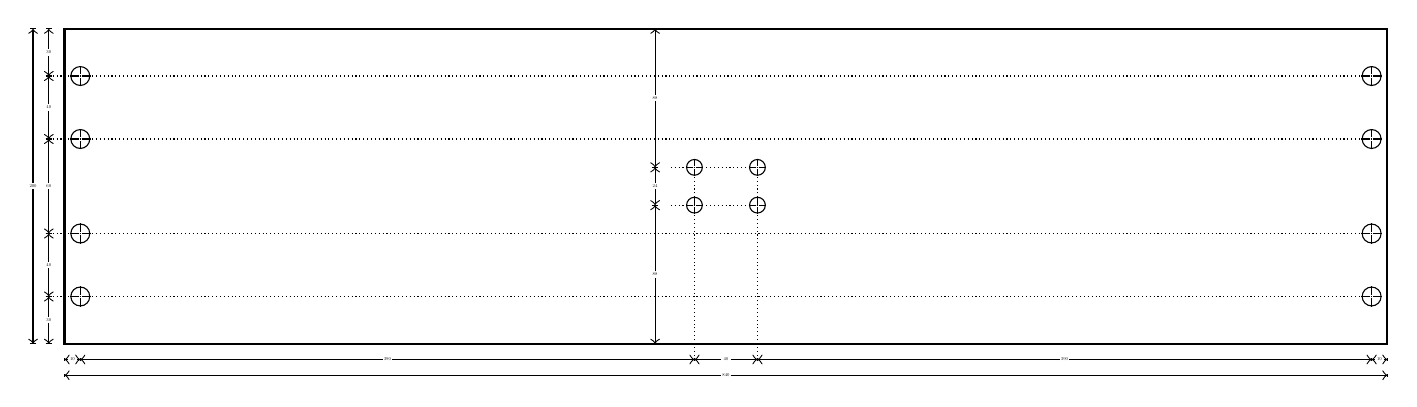
\begin{tikzpicture}[scale=0.2, every node/.style={scale=0.2}]
	% 84cm x 20cm x 12mm
	% scale 1:5
	\draw[thick] (0, 0) rectangle (84, 20);
	\hole{1}{3}{6};
	\hole{1}{7}{6};
	\hole{1}{13}{6};
	\hole{1}{17}{6};
	
	\hole{83}{3}{6};
	\hole{83}{7}{6};
	\hole{83}{13}{6};
	\hole{83}{17}{6};
	
	\hole{40}{8.8}{5};
	\hole{40}{11.2}{5};
	\hole{44}{8.8}{5};
	\hole{44}{11.2}{5};
	
	\dimsh{0}{1}{-1};
	\dimsh{1}{40}{-1};
	\dimsh{40}{44}{-1};
	\dimsh{44}{83}{-1};
	\dimsh{83}{84}{-1};
	\dimsh{0}{84}{-2};
	
	\draw[densely dotted] (40, -1) -- (40, 8.3);
	\draw[densely dotted] (40, 9.3) -- (40, 10.7);
	\draw[densely dotted] (44, -1) -- (44, 8.3);
	\draw[densely dotted] (44, 9.3) -- (44, 10.7);
	
	\dimsv{0}{3}{-1};
	\dimsv{3}{7}{-1};
	\dimsv{7}{13}{-1};
	\dimsv{13}{17}{-1};
	\dimsv{17}{20}{-1};
	\dimsv{0}{20}{-2};
	
	\draw[densely dotted] (-1, 3) -- (0.5, 3);
	\draw[densely dotted] (1.5, 3) -- (82.5, 3);
	\draw[densely dotted] (-1, 7) -- (0.5, 7);
	\draw[densely dotted] (1.5, 7) -- (82.5, 7);
	\draw[densely dotted] (-1, 13) -- (0.5, 13);
	\draw[densely dotted] (1.5, 13) -- (82.5, 13);
	\draw[densely dotted] (-1, 17) -- (0.5, 17);
	\draw[densely dotted] (1.5, 17) -- (82.5, 17);
	
	\dimsv{0}{8.8}{37.5};
	\dimsv{8.8}{11.2}{37.5};
	\dimsv{11.2}{20}{37.5};
	
	\draw[densely dotted] (38.5, 8.8) -- (39.5, 8.8);
	\draw[densely dotted] (40.5, 8.8) -- (44.5, 8.8);
	\draw[densely dotted] (38.5, 11.2) -- (39.5, 11.2);
	\draw[densely dotted] (40.5, 11.2) -- (44.5, 11.2);

	\end{tikzpicture}
\caption{Base Plate.}
\label{fig:base_plate}
\end{figure}
\begin{figure}[h]
	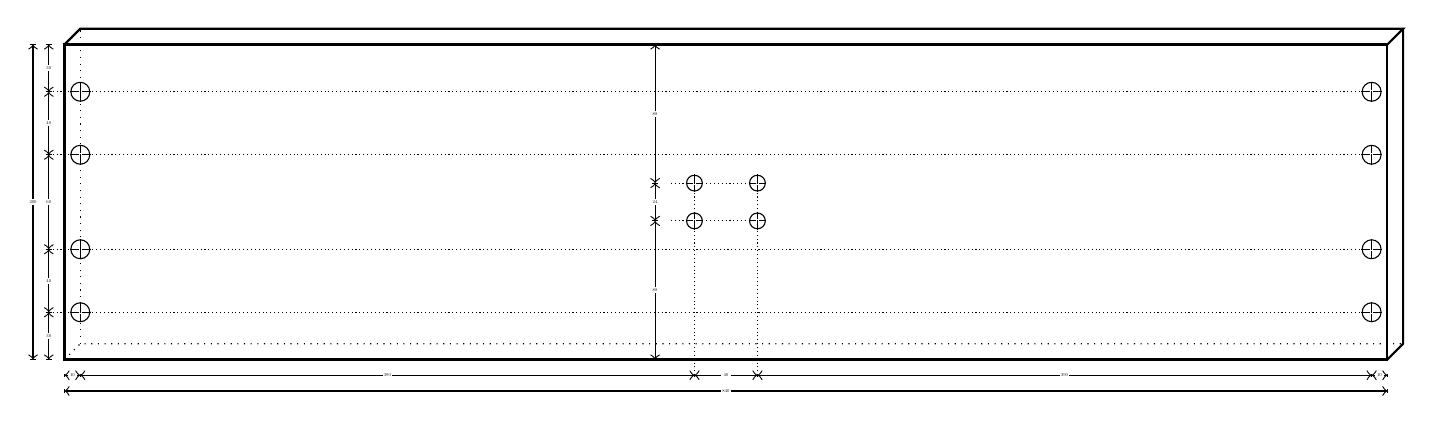
\begin{tikzpicture}[scale=0.2, every node/.style={scale=0.2}]
	% 84cm x 20cm x 12mm
	% scale 1:5
	\draw[thick] (0, 0) rectangle (84, 20);
	\draw[thick] (0, 20) -- (1, 21) -- (85, 21) -- (84, 20);
	\draw[thick] (85, 21) -- (85, 1) -- (84, 0);
	\draw[dotted] (0, 0) -- (1, 1) -- (85, 1);
	\draw[dotted] (1, 1) -- (1, 21);
	\hole{1}{3}{6};
	\hole{1}{7}{6};
	\hole{1}{13}{6};
	\hole{1}{17}{6};
	
	\hole{83}{3}{6};
	\hole{83}{7}{6};
	\hole{83}{13}{6};
	\hole{83}{17}{6};
	
	\hole{40}{8.8}{5};
	\hole{40}{11.2}{5};
	\hole{44}{8.8}{5};
	\hole{44}{11.2}{5};
	
	\dimsh{0}{1}{-1};
	\dimsh{1}{40}{-1};
	\dimsh{40}{44}{-1};
	\dimsh{44}{83}{-1};
	\dimsh{83}{84}{-1};
	\dimsh{0}{84}{-2};
	
	\draw[densely dotted] (40, -1) -- (40, 8.3);
	\draw[densely dotted] (40, 9.3) -- (40, 10.7);
	\draw[densely dotted] (44, -1) -- (44, 8.3);
	\draw[densely dotted] (44, 9.3) -- (44, 10.7);
	
	\dimsv{0}{3}{-1};
	\dimsv{3}{7}{-1};
	\dimsv{7}{13}{-1};
	\dimsv{13}{17}{-1};
	\dimsv{17}{20}{-1};
	\dimsv{0}{20}{-2};
	
	\draw[densely dotted] (-1, 3) -- (0.5, 3);
	\draw[densely dotted] (1.5, 3) -- (82.5, 3);
	\draw[densely dotted] (-1, 7) -- (0.5, 7);
	\draw[densely dotted] (1.5, 7) -- (82.5, 7);
	\draw[densely dotted] (-1, 13) -- (0.5, 13);
	\draw[densely dotted] (1.5, 13) -- (82.5, 13);
	\draw[densely dotted] (-1, 17) -- (0.5, 17);
	\draw[densely dotted] (1.5, 17) -- (82.5, 17);
	
	\dimsv{0}{8.8}{37.5};
	\dimsv{8.8}{11.2}{37.5};
	\dimsv{11.2}{20}{37.5};
	
	\draw[densely dotted] (38.5, 8.8) -- (39.5, 8.8);
	\draw[densely dotted] (40.5, 8.8) -- (44.5, 8.8);
	\draw[densely dotted] (38.5, 11.2) -- (39.5, 11.2);
	\draw[densely dotted] (40.5, 11.2) -- (44.5, 11.2);
	
	\end{tikzpicture}
	\caption{Base Plate 3D.}
	\label{fig:base_plate_3d}
\end{figure}
\subsubsection{Front Plate}
\begin{figure}[h]
	\begin{tikzpicture}[scale=0.8, every node/.style={scale=0.8}]
	% 19cm x 16cm x 12mm
	% scale 1:5
	\draw[thick] (0, 0) rectangle (19, 16);
	\hole{1.5}{12}{3};
	\hole{5.5}{12}{3};
	\hole{13.5}{12}{3};
	\hole{17.5}{12}{3};
	
	\hole{9.5}{8}{13};
	
	\hole{7.125}{5.625}{2.5};
	\hole{7.125}{10.375}{2.5};
	\hole{11.875}{5.625}{2.5};
	\hole{11.875}{10.375}{2.5};
	
	\end{tikzpicture}
	\caption{Front Plate.}
	\label{fig:front_plate}
\end{figure}
\begin{figure}[h]
	\begin{tikzpicture}[scale=0.8, every node/.style={scale=0.8}]
	% 19cm x 16cm x 12mm
	% scale 1:5
	\draw[thick] (0, 0) rectangle (19, 16);
	\draw[thick] (0, 16) -- (1, 17) -- (20, 17) -- (19, 16);
	\draw[thick] (20, 17) -- (20, 1) -- (19, 0);
	\draw[dotted] (0, 0) -- (1, 1) -- (20, 1);
	\draw[dotted] (1, 1) -- (1, 17);
	
	\hole{1.5}{12}{3};
	\hole{5.5}{12}{3};
	\hole{13.5}{12}{3};
	\hole{17.5}{12}{3};
	
	\hole{9.5}{8}{13};
	
	\hole{7.125}{5.625}{2.5};
	\hole{7.125}{10.375}{2.5};
	\hole{11.875}{5.625}{2.5};
	\hole{11.875}{10.375}{2.5};
	
	\end{tikzpicture}
	\caption{Front Plate 3D.}
	\label{fig:front_plate_3d}
\end{figure}
\subsection{Spindle Y mount}
\subsubsection{Side Plate}
\begin{figure}[h]
	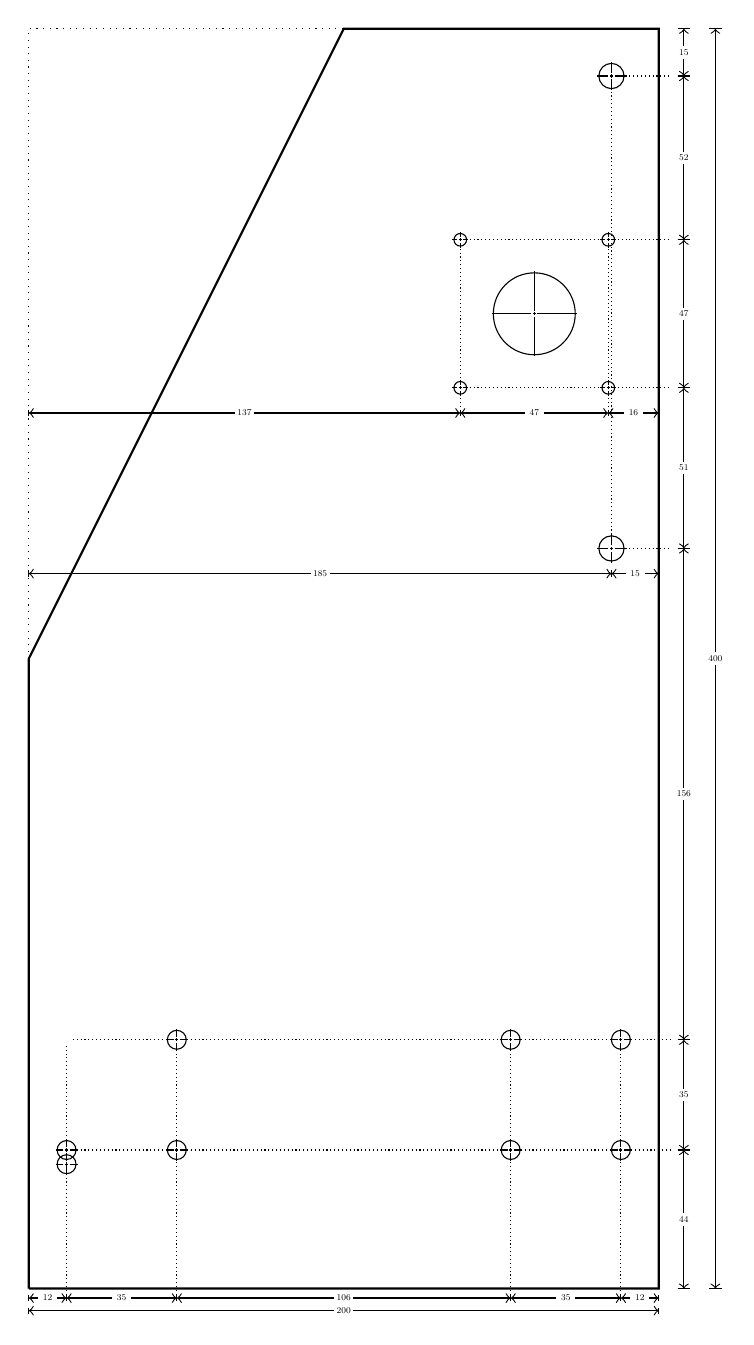
\begin{tikzpicture}[scale=0.4, every node/.style={scale=0.4}]
	% 20cm x 40cm x 20mm
	% scale 2:5
	%\draw[thick] (0, 0) rectangle (10, 20);
	\draw[thick] (0, 0) -- (20, 0) -- (20, 40) -- (10, 40) -- (0, 20) -- (0, 0);
	\draw[dotted] (0, 20) -- (0, 40) -- (10, 40);
	\hole{1.2}{4.4}{3};
	\hole{1.2}{3.95}{3};
	\hole{4.7}{4.4}{3};
	\hole{4.7}{7.9}{3};
	
	\hole{15.3}{4.4}{3};
	\hole{15.3}{7.9}{3};
	\hole{18.8}{4.4}{3};
	\hole{18.8}{7.9}{3};
	
	\hole{18.5}{23.5}{4};
	\hole{18.5}{38.5}{4};
	
	\hole{13.7}{28.6}{2};
	\hole{13.7}{33.3}{2};
	\hole{18.4}{28.6}{2};
	\hole{18.4}{33.3}{2};
	
	\hole{16.05}{30.95}{13};
	
	
	\dimsh{0}{1.2}{-0.3};
	\dimsh{1.2}{4.7}{-0.3};
	\dimsh{4.7}{15.3}{-0.3};
	\dimsh{15.3}{18.8}{-0.3};
	\dimsh{18.8}{20}{-0.3};
	\dimsh{0}{20}{-0.7};
	
	\draw[densely dotted] (1.2, -0.2) -- (1.2, 4.2);
	\draw[densely dotted] (1.2, 4.6) -- (1.2, 7.7);
	\draw[densely dotted] (4.7, -0.2) -- (4.7, 4.2);
	\draw[densely dotted] (4.7, 4.6) -- (4.7, 7.7);
	\draw[densely dotted] (15.3, -0.2) -- (15.3, 4.2);
	\draw[densely dotted] (15.3, 4.6) -- (15.3, 7.7);
	\draw[densely dotted] (18.8, -0.2) -- (18.8, 4.2);
	\draw[densely dotted] (18.8, 4.6) -- (18.8, 7.7);
	
	\dimsv{0}{4.4}{20.8};
	\dimsv{4.4}{7.9}{20.8};
	\dimsv{7.9}{23.5}{20.8};
	\dimsv{23.5}{28.6}{20.8};
	\dimsv{28.6}{33.3}{20.8};
	\dimsv{33.3}{38.5}{20.8};
	\dimsv{38.5}{40}{20.8};
	\dimsv{0}{40}{21.8};
	
	\draw[densely dotted] (1.4, 4.4) -- (4.5, 4.4);
	\draw[densely dotted] (4.9, 4.4) -- (15.1, 4.4);
	\draw[densely dotted] (15.5, 4.4) -- (18.6, 4.4);
	\draw[densely dotted] (19, 4.4) -- (20.4, 4.4);
	\draw[densely dotted] (1.4, 7.9) -- (4.5, 7.9);
	\draw[densely dotted] (4.9, 7.9) -- (15.1, 7.9);
	\draw[densely dotted] (15.5, 7.9) -- (18.6, 7.9);
	\draw[densely dotted] (19, 7.9) -- (20.4, 7.9);
	
	\draw[densely dotted] (18.7, 23.5) -- (20.4, 23.5);
	\draw[densely dotted] (18.7, 38.5) -- (20.4, 38.5);
	
	\dimsh{0}{18.5}{22.7};
	\dimsh{18.5}{20}{22.7};
	
	\draw[densely dotted] (18.5, 23.7) -- (18.5, 38.3);
	
	\draw[densely dotted] (14, 28.6) -- (18.3, 28.6);
	\draw[densely dotted] (18.7, 28.6) -- (20.4, 28.6);
	\draw[densely dotted] (14, 33.3) -- (18.3, 33.3);
	\draw[densely dotted] (18.7, 33.3) -- (20.4, 33.3);
	
	\dimsh{0}{13.7}{27.8};
	\dimsh{13.7}{18.4}{27.8};
	\dimsh{18.4}{20}{27.8};
	
	\draw[densely dotted] (13.7, 28) -- (13.7, 28.4);
	\draw[densely dotted] (13.7, 28.8) -- (13.7, 33.1);
	\draw[densely dotted] (18.4, 28) -- (18.4, 28.4);
	\draw[densely dotted] (18.4, 28.8) -- (18.4, 33.1);
	
	
	
	\end{tikzpicture}
\caption{Side Plate.}
\label{fig:side_plate}
\end{figure}

\begin{figure}[h]
	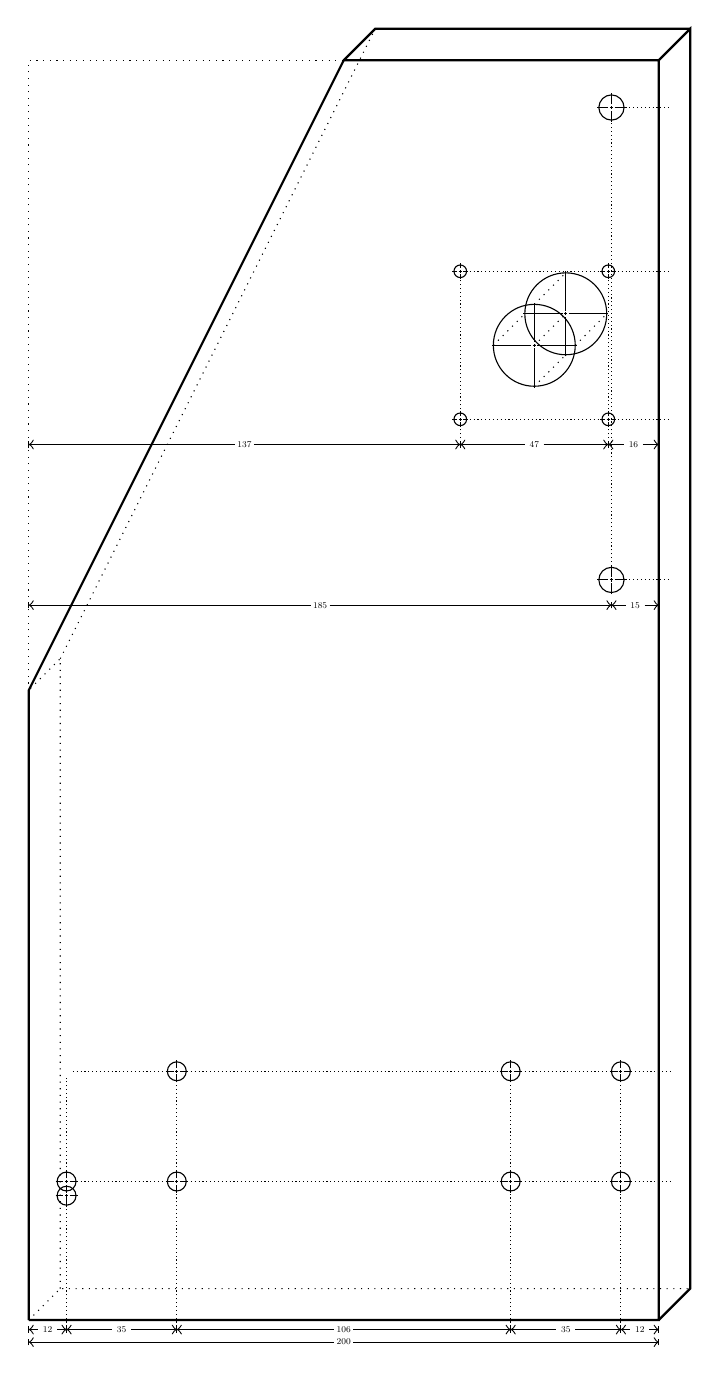
\begin{tikzpicture}[scale=0.4, every node/.style={scale=0.4}]
	% 20cm x 40cm x 20mm
	% scale 2:5
	%\draw[thick] (0, 0) rectangle (10, 20);
	\draw[thick] (0, 0) -- (20, 0) -- (20, 40) -- (10, 40) -- (0, 20) -- (0, 0);
	\draw[thick] (20, 0) -- (21, 1) -- (21, 41)-- (20, 40);
	\draw[thick] (10, 40) -- (11, 41) -- (21, 41);
	\draw[dotted] (0, 0) -- (1, 1) -- (21, 1);
	\draw[dotted] (1, 1) -- (1, 21) -- (0, 20);
	\draw[dotted] (1, 21) -- (11, 41);
	\draw[dotted] (0, 20) -- (0, 40) -- (10, 40);
	\hole{1.2}{4.4}{3};
	\hole{1.2}{3.95}{3};
	\hole{4.7}{4.4}{3};
	\hole{4.7}{7.9}{3};
	
	\hole{15.3}{4.4}{3};
	\hole{15.3}{7.9}{3};
	\hole{18.8}{4.4}{3};
	\hole{18.8}{7.9}{3};
	
	\hole{18.5}{23.5}{4};
	\hole{18.5}{38.5}{4};
	
	\hole{13.7}{28.6}{2};
	\hole{13.7}{33.3}{2};
	\hole{18.4}{28.6}{2};
	\hole{18.4}{33.3}{2};
	
	\hole{16.05}{30.95}{13};
	\hole{17.05}{31.95}{13};
	\draw[dotted] (16.05, 30.95) -- (17.05, 31.95);
	\draw[dotted] (14.75, 30.95) -- (15.75, 31.95);
	\draw[dotted] (17.35, 30.95) -- (18.35, 31.95);
	\draw[dotted] (16.05, 29.65) -- (17.05, 30.65);
	\draw[dotted] (16.05, 32.25) -- (17.05, 33.25);
	
	
	\dimsh{0}{1.2}{-0.3};
	\dimsh{1.2}{4.7}{-0.3};
	\dimsh{4.7}{15.3}{-0.3};
	\dimsh{15.3}{18.8}{-0.3};
	\dimsh{18.8}{20}{-0.3};
	\dimsh{0}{20}{-0.7};
	
	\draw[densely dotted] (1.2, -0.2) -- (1.2, 4.2);
	\draw[densely dotted] (1.2, 4.6) -- (1.2, 7.7);
	\draw[densely dotted] (4.7, -0.2) -- (4.7, 4.2);
	\draw[densely dotted] (4.7, 4.6) -- (4.7, 7.7);
	\draw[densely dotted] (15.3, -0.2) -- (15.3, 4.2);
	\draw[densely dotted] (15.3, 4.6) -- (15.3, 7.7);
	\draw[densely dotted] (18.8, -0.2) -- (18.8, 4.2);
	\draw[densely dotted] (18.8, 4.6) -- (18.8, 7.7);
	
	%\dimsv{0}{4.4}{20.8};
	%\dimsv{4.4}{7.9}{20.8};
	%\dimsv{7.9}{23.5}{20.8};
	%\dimsv{23.5}{28.6}{20.8};
	%\dimsv{28.6}{33.3}{20.8};
	%\dimsv{33.3}{38.5}{20.8};
	%\dimsv{38.5}{40}{20.8};
	%\dimsv{0}{40}{21.8};
	
	\draw[densely dotted] (1.4, 4.4) -- (4.5, 4.4);
	\draw[densely dotted] (4.9, 4.4) -- (15.1, 4.4);
	\draw[densely dotted] (15.5, 4.4) -- (18.6, 4.4);
	\draw[densely dotted] (19, 4.4) -- (20.4, 4.4);
	\draw[densely dotted] (1.4, 7.9) -- (4.5, 7.9);
	\draw[densely dotted] (4.9, 7.9) -- (15.1, 7.9);
	\draw[densely dotted] (15.5, 7.9) -- (18.6, 7.9);
	\draw[densely dotted] (19, 7.9) -- (20.4, 7.9);
	
	\draw[densely dotted] (18.7, 23.5) -- (20.4, 23.5);
	\draw[densely dotted] (18.7, 38.5) -- (20.4, 38.5);
	
	\dimsh{0}{18.5}{22.7};
	\dimsh{18.5}{20}{22.7};
	
	\draw[densely dotted] (18.5, 23.7) -- (18.5, 38.3);
	
	\draw[densely dotted] (14, 28.6) -- (18.3, 28.6);
	\draw[densely dotted] (18.7, 28.6) -- (20.4, 28.6);
	\draw[densely dotted] (14, 33.3) -- (18.3, 33.3);
	\draw[densely dotted] (18.7, 33.3) -- (20.4, 33.3);
	
	\dimsh{0}{13.7}{27.8};
	\dimsh{13.7}{18.4}{27.8};
	\dimsh{18.4}{20}{27.8};
	
	\draw[densely dotted] (13.7, 28) -- (13.7, 28.4);
	\draw[densely dotted] (13.7, 28.8) -- (13.7, 33.1);
	\draw[densely dotted] (18.4, 28) -- (18.4, 28.4);
	\draw[densely dotted] (18.4, 28.8) -- (18.4, 33.1);
	
	
	
	\end{tikzpicture}
	\caption{Side Plate 3D.}
	\label{fig:side_plate_3d}
\end{figure}

\subsubsection{Rear Plate}
\begin{figure}[h]
	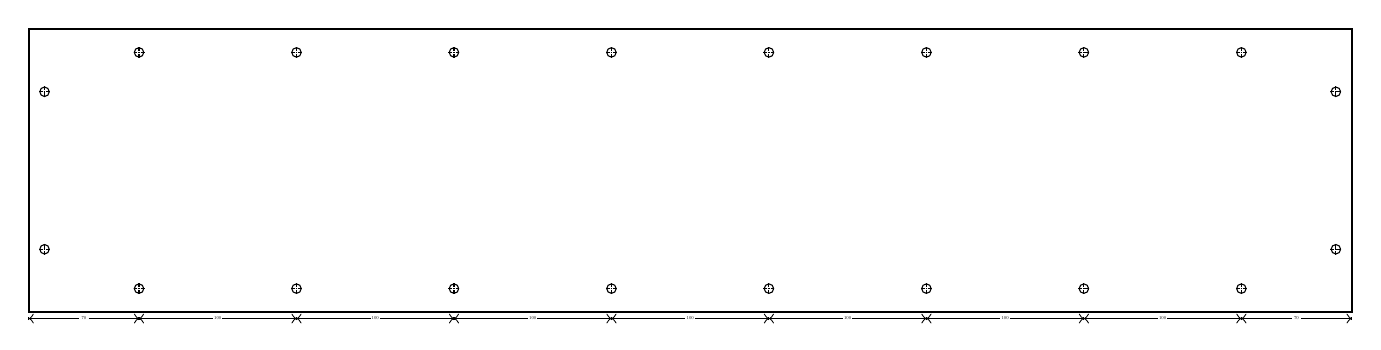
\begin{tikzpicture}[scale=0.2, every node/.style={scale=0.2}]
	% 84cm x 18cm x 10mm
	% scale 1:5
	\draw[thick] (0, 0) rectangle (84, 18);
	\hole{1}{4}{3};
	\hole{1}{14}{3};
	\hole{83}{4}{3};
	\hole{83}{14}{3};
	
	\hole{7}{1.5}{3};
	\hole{7}{16.5}{3};
	\hole{17}{1.5}{3};
	\hole{17}{16.5}{3};
	\hole{27}{1.5}{3};
	\hole{27}{16.5}{3};
	\hole{37}{1.5}{3};
	\hole{37}{16.5}{3};
	\hole{47}{1.5}{3};
	\hole{47}{16.5}{3};
	\hole{57}{1.5}{3};
	\hole{57}{16.5}{3};
	\hole{67}{1.5}{3};
	\hole{67}{16.5}{3};
	\hole{77}{1.5}{3};
	\hole{77}{16.5}{3};
	
	\dimsh{0}{7}{-0.4};
	\dimsh{7}{17}{-0.4};
	\dimsh{17}{27}{-0.4};
	\dimsh{27}{37}{-0.4};
	\dimsh{37}{47}{-0.4};
	\dimsh{47}{57}{-0.4};
	\dimsh{57}{67}{-0.4};
	\dimsh{67}{77}{-0.4};
	\dimsh{77}{84}{-0.4};
	\end{tikzpicture}
\caption{Rear Plate.}
\label{fig:rear_plate}
\end{figure}
\begin{figure}[h]
	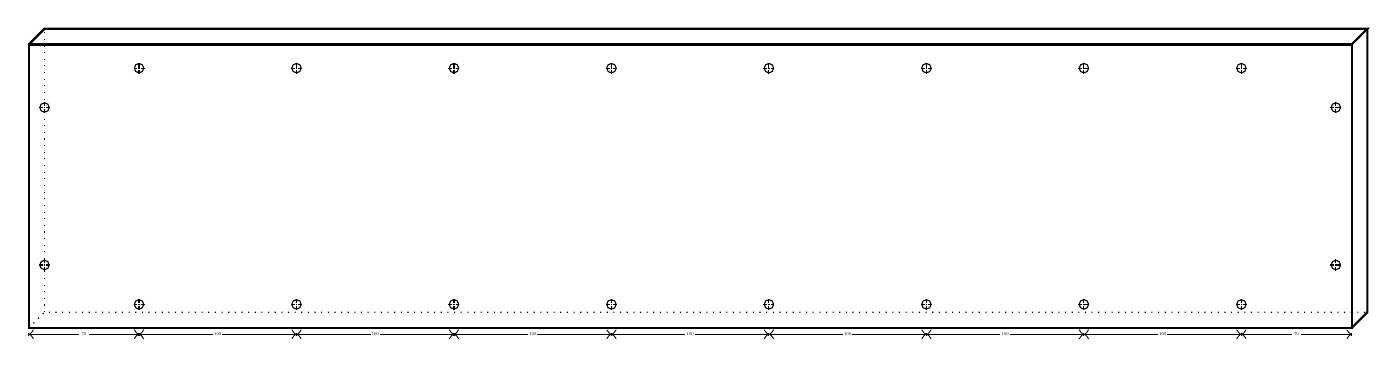
\begin{tikzpicture}[scale=0.2, every node/.style={scale=0.2}]
	% 84cm x 18cm x 10mm
	% scale 1:5
	\draw[thick] (0, 0) rectangle (84, 18);
	\draw[thick] (0, 18) -- (1, 19) -- (85, 19) -- (84, 18);
	\draw[thick] (85, 19) -- (85, 1) -- (84, 0);
	\draw[dotted] (0, 0) -- (1, 1) -- (85, 1);
	\draw[dotted] (1, 1) -- (1, 19);
	\hole{1}{4}{3};
	\hole{1}{14}{3};
	\hole{83}{4}{3};
	\hole{83}{14}{3};
	
	\hole{7}{1.5}{3};
	\hole{7}{16.5}{3};
	\hole{17}{1.5}{3};
	\hole{17}{16.5}{3};
	\hole{27}{1.5}{3};
	\hole{27}{16.5}{3};
	\hole{37}{1.5}{3};
	\hole{37}{16.5}{3};
	\hole{47}{1.5}{3};
	\hole{47}{16.5}{3};
	\hole{57}{1.5}{3};
	\hole{57}{16.5}{3};
	\hole{67}{1.5}{3};
	\hole{67}{16.5}{3};
	\hole{77}{1.5}{3};
	\hole{77}{16.5}{3};
	
	\dimsh{0}{7}{-0.4};
	\dimsh{7}{17}{-0.4};
	\dimsh{17}{27}{-0.4};
	\dimsh{27}{37}{-0.4};
	\dimsh{37}{47}{-0.4};
	\dimsh{47}{57}{-0.4};
	\dimsh{57}{67}{-0.4};
	\dimsh{67}{77}{-0.4};
	\dimsh{77}{84}{-0.4};
	\end{tikzpicture}
	\caption{Rear Plate 3D.}
	\label{fig:rear_plate_3d}
\end{figure}
\subsubsection{Rear Mount}
KPF-S 20 has been used as linear mount.
\begin{figure}[h]
	\begin{tikzpicture}[scale=0.6, every node/.style={scale=0.6}]
	% 16cm x 30cm x 15mm
	% scale 1:2
	\draw[thick] (0, 0) rectangle (16, 30);
	% horizontal waggon mount - lower
	\hole{2}{1.8}{3};
	\hole{2}{5}{3};
	\hole{5.6}{1.8}{3};
	\hole{5.6}{5}{3};
	\hole{10.4}{1.8}{3};
	\hole{10.4}{5}{3};
	\hole{14}{1.8}{3};
	\hole{14}{5}{3};
	% horizontal waggon mount - upper
	\hole{2}{16.8}{3};
	\hole{2}{20}{3};
	\hole{5.6}{16.8}{3};
	\hole{5.6}{20}{3};
	\hole{10.4}{16.8}{3};
	\hole{10.4}{20}{3};
	\hole{14}{16.8}{3};
	\hole{14}{20}{3};
	% horizontal spindle mount
	\hole{6.2}{8.9}{3};
	\hole{6.2}{12.9}{3};
	\hole{8.6}{8.9}{3};
	\hole{8.6}{12.9}{3};
	% vertical waggon mount - lower
	\hole{0.8}{8}{3};
	\hole{0.8}{11.6}{3};
	\hole{4}{8}{3};
	\hole{4}{11.6}{3};
	\hole{12}{8}{3};
	\hole{12}{11.6}{3};
	\hole{15.2}{8}{3};
	\hole{15.2}{11.6}{3};
	% vertical waggon mount - upper
	\hole{0.8}{23}{3};
	\hole{0.8}{26.6}{3};
	\hole{4}{23}{3};
	\hole{4}{26.6}{3};
	\hole{12}{23}{3};
	\hole{12}{26.6}{3};
	\hole{15.2}{23}{3};
	\hole{15.2}{26.6}{3};
	% vertical spindle mount
	\hole{6}{21.6}{3};
	\hole{6}{24}{3};
	\hole{10}{21.6}{3};
	\hole{10}{24}{3};
	
	\end{tikzpicture}
	\caption{Rear Mount.}
	\label{fig:rear_mount}
\end{figure}
\begin{figure}[h]
	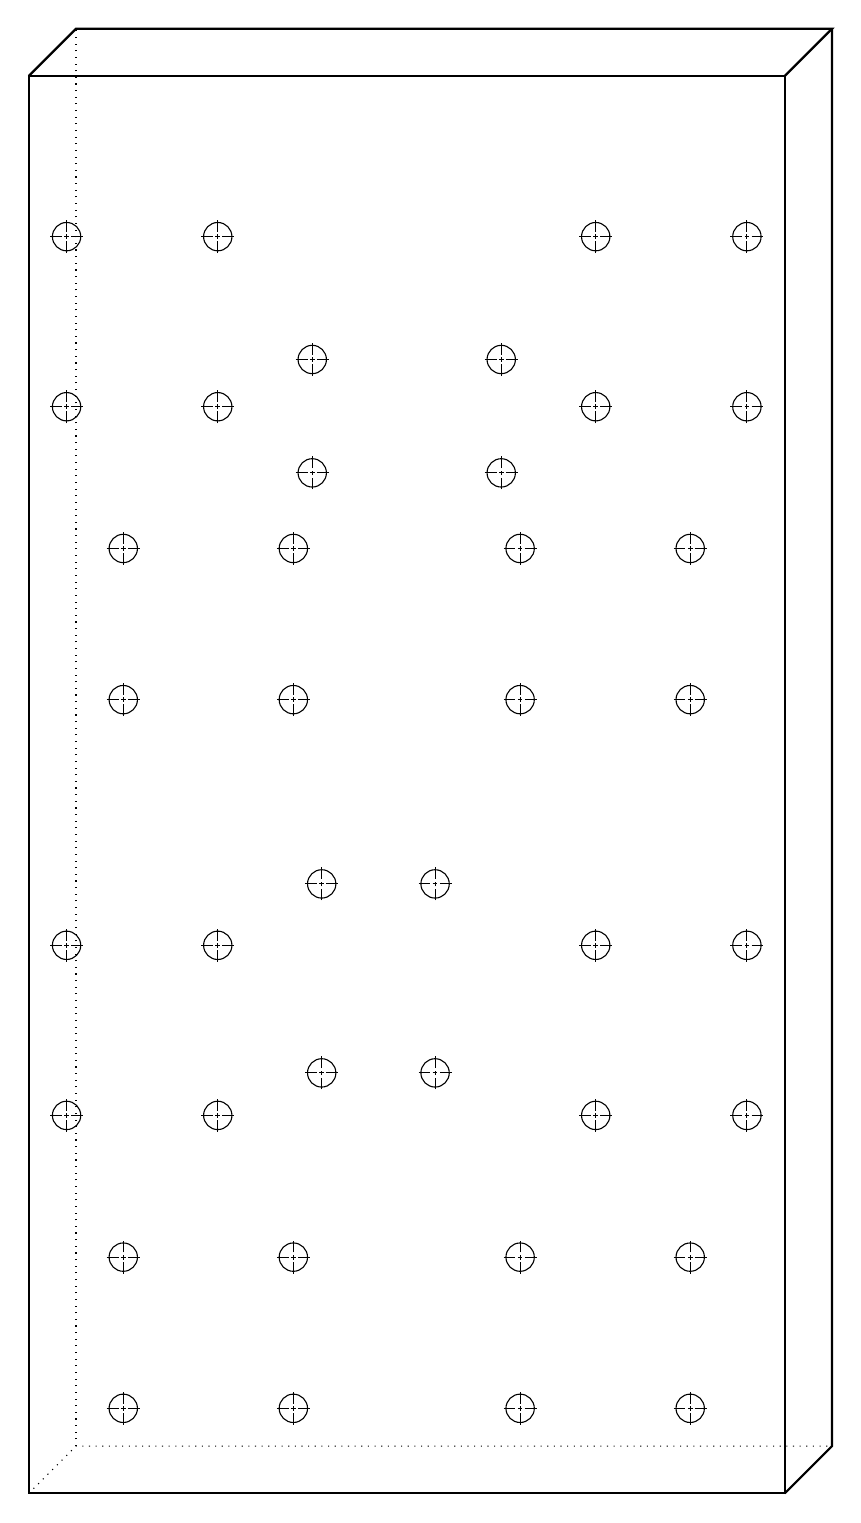
\begin{tikzpicture}[scale=0.6, every node/.style={scale=0.6}]
	% 16cm x 30cm x 15mm
	% scale 1:2
	\draw[thick] (0, 0) rectangle (16, 30);
	\draw[thick] (0, 30) -- (1, 31) -- (17, 31) -- (16, 30);
	\draw[thick] (17, 31) -- (17, 1) -- (16, 0);
	\draw[dotted] (0, 0) -- (1, 1) -- (17, 1);
	\draw[dotted] (1, 1) -- (1, 31);
	% horizontal waggon mount - lower
	\hole{2}{1.8}{3};
	\hole{2}{5}{3};
	\hole{5.6}{1.8}{3};
	\hole{5.6}{5}{3};
	\hole{10.4}{1.8}{3};
	\hole{10.4}{5}{3};
	\hole{14}{1.8}{3};
	\hole{14}{5}{3};
	% horizontal waggon mount - upper
	\hole{2}{16.8}{3};
	\hole{2}{20}{3};
	\hole{5.6}{16.8}{3};
	\hole{5.6}{20}{3};
	\hole{10.4}{16.8}{3};
	\hole{10.4}{20}{3};
	\hole{14}{16.8}{3};
	\hole{14}{20}{3};
	% horizontal spindle mount
	\hole{6.2}{8.9}{3};
	\hole{6.2}{12.9}{3};
	\hole{8.6}{8.9}{3};
	\hole{8.6}{12.9}{3};
	% vertical waggon mount - lower
	\hole{0.8}{8}{3};
	\hole{0.8}{11.6}{3};
	\hole{4}{8}{3};
	\hole{4}{11.6}{3};
	\hole{12}{8}{3};
	\hole{12}{11.6}{3};
	\hole{15.2}{8}{3};
	\hole{15.2}{11.6}{3};
	% vertical waggon mount - upper
	\hole{0.8}{23}{3};
	\hole{0.8}{26.6}{3};
	\hole{4}{23}{3};
	\hole{4}{26.6}{3};
	\hole{12}{23}{3};
	\hole{12}{26.6}{3};
	\hole{15.2}{23}{3};
	\hole{15.2}{26.6}{3};
	% vertical spindle mount
	\hole{6}{21.6}{3};
	\hole{6}{24}{3};
	\hole{10}{21.6}{3};
	\hole{10}{24}{3};
	
	\end{tikzpicture}
	\caption{Rear Mount 3D.}
	\label{fig:rear_mount_3d}
\end{figure}
\subsection{Spindle Z Mount}
\subsubsection{Main}
\begin{figure}[h]
	\begin{tikzpicture}[scale=0.4, every node/.style={scale=0.4}]
	% 16cm x 40cm x 15mm
	% scale 2:5
	\draw[thick] (0, 0) rectangle (16, 40);
	\hole{4.5}{1.7}{3.5};
	\hole{11.5}{1.7}{3.5};
	\hole{4.5}{3}{3.5};
	\hole{4.5}{6.3}{3.5};
	\hole{11.5}{3}{3.5};
	\hole{11.5}{6.3}{3.5};
	
	
	\hole{2.4}{2}{3};
	\hole{2.4}{8}{3};
	\hole{2.4}{14}{3};
	\hole{2.4}{20}{3};
	\hole{2.4}{26}{3};
	\hole{2.4}{32}{3};
	\hole{2.4}{38}{3};
	\hole{13.6}{2}{3};
	\hole{13.6}{8}{3};
	\hole{13.6}{14}{3};
	\hole{13.6}{20}{3};
	\hole{13.6}{26}{3};
	\hole{13.6}{32}{3};
	\hole{13.6}{38}{3};
	
	\end{tikzpicture}
	\caption{Spindle Z Mount - Main.}
	\label{fig:spindle_z_mount_main}
\end{figure}
\begin{figure}[h]
	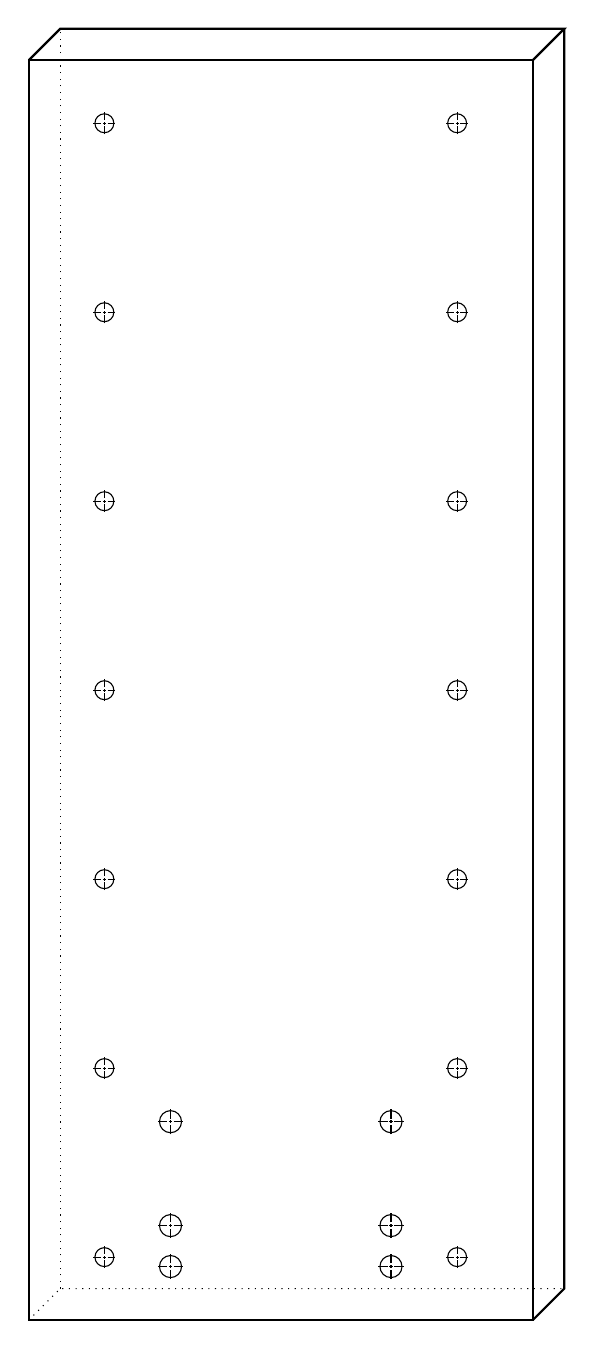
\begin{tikzpicture}[scale=0.4, every node/.style={scale=0.4}]
	% 16cm x 40cm x 15mm
	% scale 2:5
	\draw[thick] (0, 0) rectangle (16, 40);
	\draw[thick] (0, 40) -- (1, 41) -- (17, 41) -- (16, 40);
	\draw[thick] (17, 41) -- (17, 1) -- (16, 0);
	\draw[dotted] (0, 0) -- (1, 1) -- (17, 1);
	\draw[dotted] (1, 1) -- (1, 41);
	\hole{4.5}{1.7}{3.5};
	\hole{11.5}{1.7}{3.5};
	\hole{4.5}{3}{3.5};
	\hole{4.5}{6.3}{3.5};
	\hole{11.5}{3}{3.5};
	\hole{11.5}{6.3}{3.5};
	
	
	\hole{2.4}{2}{3};
	\hole{2.4}{8}{3};
	\hole{2.4}{14}{3};
	\hole{2.4}{20}{3};
	\hole{2.4}{26}{3};
	\hole{2.4}{32}{3};
	\hole{2.4}{38}{3};
	\hole{13.6}{2}{3};
	\hole{13.6}{8}{3};
	\hole{13.6}{14}{3};
	\hole{13.6}{20}{3};
	\hole{13.6}{26}{3};
	\hole{13.6}{32}{3};
	\hole{13.6}{38}{3};
	\end{tikzpicture}
	\caption{Spindle Z Mount - Main 3D.}
	\label{fig:spindle_z_mount_main_3d}
\end{figure}
\subsubsection{Upper}
\begin{figure}[h]
	\begin{tikzpicture}
	% 16cm x 8cm x 15mm
	% scale 1:1
	\draw[thick] (0, 0) rectangle (16, 8);
	\hole{1}{0.75}{3};
	\hole{4}{0.75}{3};
	\hole{12}{0.75}{3};
	\hole{15}{0.75}{3};
	
	\hole{2.4}{2.5}{3.5};
	\hole{13.6}{2.5}{3.5};
	
	\hole{8}{4.5}{13};
	
	\hole{5.8}{4.5}{2.5};
	\hole{8}{2.3}{2.5};
	\hole{8}{6.7}{2.5};
	\hole{10.2}{4.5}{2.5};
	
	\hole{5.625}{2.125}{2.5};
	\hole{5.625}{6.875}{2.5};
	\hole{10.375}{2.125}{2.5};
	\hole{10.375}{6.875}{2.5};
	\end{tikzpicture}
	\caption{Spindle Z Mount - Upper.}
	\label{fig:spindle_z_mount_upper}
\end{figure}
\begin{figure}[h]
	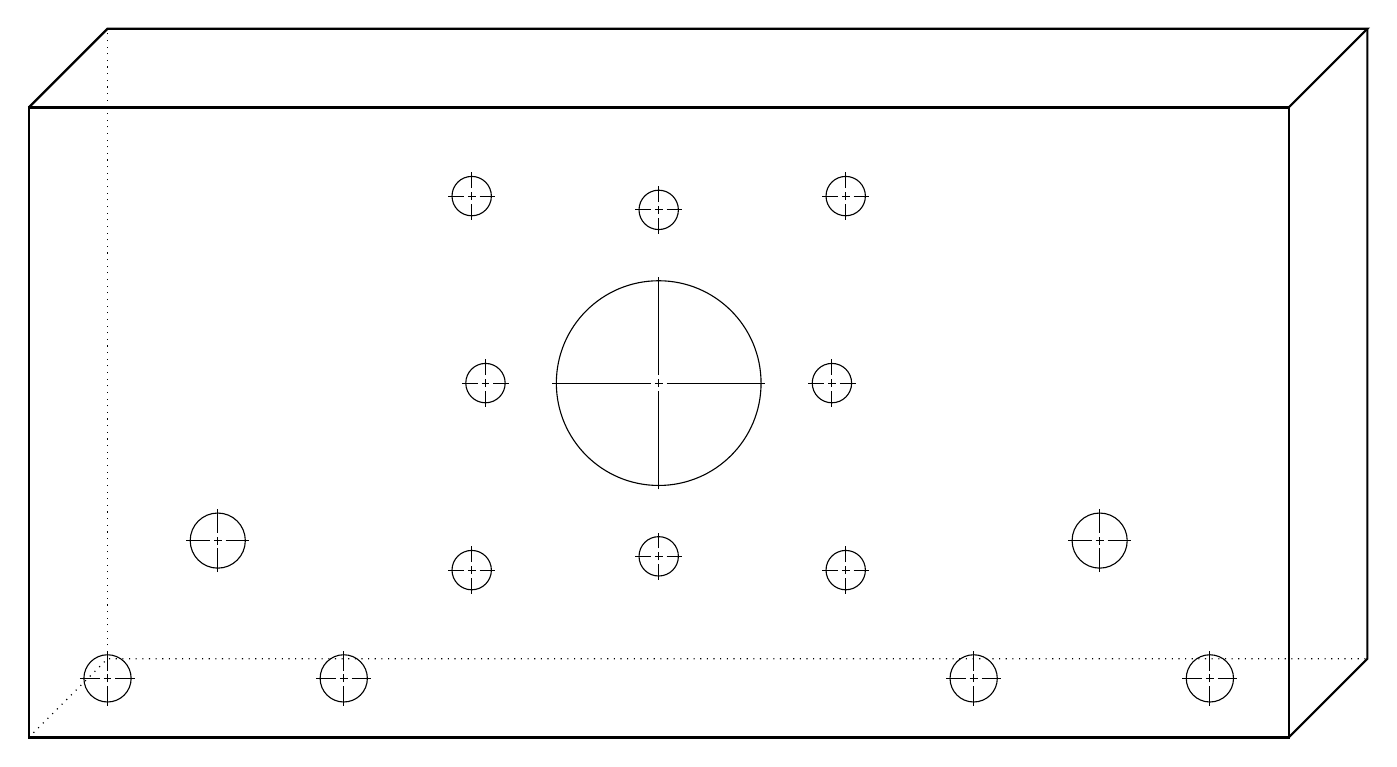
\begin{tikzpicture}
	% 16cm x 8cm x 15mm
	% scale 1:1
	\draw[thick] (0, 0) rectangle (16, 8);
	\draw[thick] (0, 8) -- (1, 9) -- (17, 9) -- (16, 8);
	\draw[thick] (17, 9) -- (17, 1) -- (16, 0);
	\draw[dotted] (0, 0) -- (1, 1) -- (17, 1);
	\draw[dotted] (1, 1) -- (1, 9);
	\hole{1}{0.75}{3};
	\hole{4}{0.75}{3};
	\hole{12}{0.75}{3};
	\hole{15}{0.75}{3};
	
	\hole{2.4}{2.5}{3.5};
	\hole{13.6}{2.5}{3.5};
	
	\hole{8}{4.5}{13};
	
	\hole{5.8}{4.5}{2.5};
	\hole{8}{2.3}{2.5};
	\hole{8}{6.7}{2.5};
	\hole{10.2}{4.5}{2.5};
	
	\hole{5.625}{2.125}{2.5};
	\hole{5.625}{6.875}{2.5};
	\hole{10.375}{2.125}{2.5};
	\hole{10.375}{6.875}{2.5};
	\end{tikzpicture}
	\caption{Spindle Z Mount - Upper 3D.}
	\label{fig:spindle_z_mount_upper_3d}
\end{figure}
\subsubsection{Lower}
\begin{figure}[h]
	\begin{tikzpicture}
	% 9cm x 8cm x 15mm
	% scale 1:1
	\draw[thick] (0, 0) rectangle (9, 8);
	\hole{4.5}{3}{13};
	
	\hole{2.4}{3}{2.5};
	\hole{4.5}{0.9}{2.5};
	\hole{4.5}{5.1}{2.5};
	\hole{6.6}{3}{2.5};
	\end{tikzpicture}
	\caption{Spindle Z Mount - Lower.}
	\label{fig:spindle_z_mount_lower}
\end{figure}
\begin{figure}[h]
	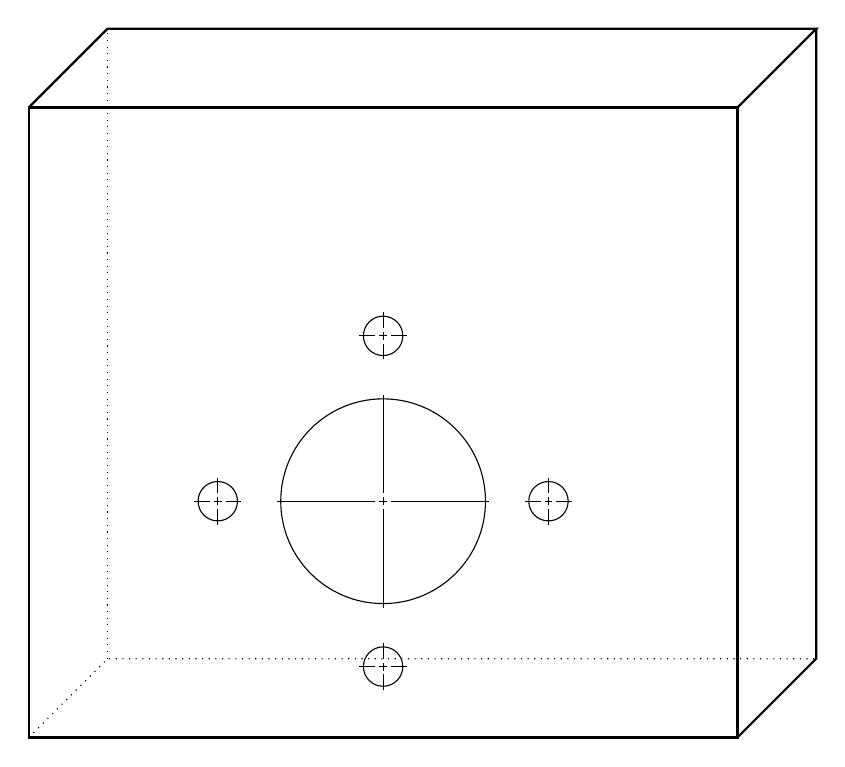
\begin{tikzpicture}
	% 9cm x 8cm x 15mm
	% scale 1:1
	\draw[thick] (0, 0) rectangle (9, 8);
	\draw[thick] (0, 8) -- (1, 9) -- (10, 9) -- (9, 8);
	\draw[thick] (10, 9) -- (10, 1) -- (9, 0);
	\draw[dotted] (0, 0) -- (1, 1) -- (10, 1);
	\draw[dotted] (1, 1) -- (1, 9);
	\hole{4.5}{3}{13};
	
	\hole{2.4}{3}{2.5};
	\hole{4.5}{0.9}{2.5};
	\hole{4.5}{5.1}{2.5};
	\hole{6.6}{3}{2.5};
	\end{tikzpicture}
	\caption{Spindle Z Mount - Lower 3D.}
	\label{fig:spindle_z_mount_lower_3d}
\end{figure}
\end{document}